
\begin{figure}[t]
    \centering
    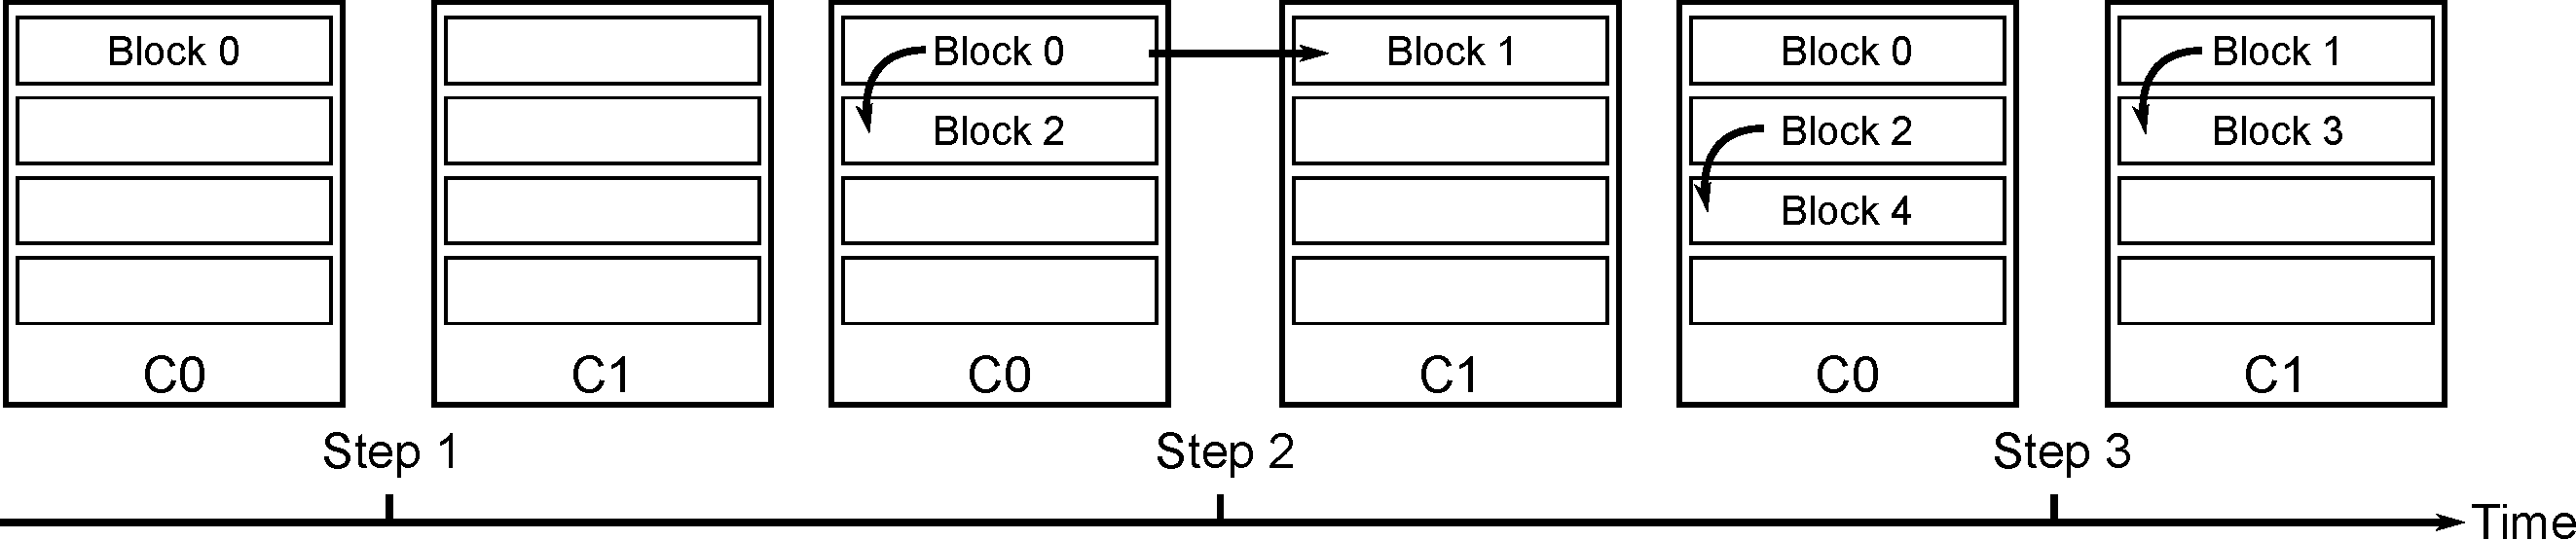
\includegraphics[width=1\textwidth]{chapter3/graphics/fetching-model.pdf}

    \caption{Example of new fetching model on a 2 core composition. Each core has 4 segments, the arrows represent the block generating the predictions. This figure shows the first 3 steps of a new core composition fetching blocks.}
    \label{fig:new_fetch_ex}
\end{figure}
Serialising block fetches in a core-composition is one of the main bottlenecks for performance when large blocks cannot be produced.
As discussed in Section~\ref{ch3:sec:bfn} this is due to the requirement that cores be full before submitting a prediction to another core.
This means that work cannot be parallelised on cores as quickly as more traditional methods such as multi-threading.
Indeed, in a multi-threaded system, cores can independently fetch blocks and thus maximize throughput easily.
A mechanism that can alleviate communication between cores is a first step in improving block throughput for core-compositions.

In this chapter, a new block-fetching scheme is introduced which reduces the amount of reliance on other cores in the composition.
This new scheme is then evaluated against the old fetching scheme on the synethtic benchmark from section~\ref{ch3:sec:bfn}.

\subsection{Independent block fetching scheme}

In a core-composition, cores should be able to fetch blocks without requiring a signal from a previous core in the same composition.
Instead, to enable maximum block throughput cores must limit communication to flushes and an initial fetch request.
This allows cores to always be fetching as long as a misprediction hasn't happened.
An initial fetch request is always necessary as only a single core is fetching the first block during a new reconfiguration of the DMP and therefore, other cores must be prompted to fetch at least one block.
However, unlike the current serial model, cores should attempt to submit a fetch signal to the next core in the composition as soon as possible to ensure that all cores are in use.
To understand how the new block mechanism behaves, it will be described in two parts.
The first part will use a concrete example of 2 cores fused, whilst the second part will generalise the mechanism to n-cores fused.

Given a 2 core-fusion \{$Core_0$,$Core_1$\} using a multi-block ahead branch predictor described by A. Seznec et al in~\cite{SeseznecMultipleBlock} the cores can make two predictions in a single cycle: one for itself and one for the next core.
Figure~\ref{fig:new_fetch_ex} gives an overview of the first few cycles of using the new block-fetching scheme with the two cores fused.
When $Core_0$ starts the composition and fetches the first block, $block_0$, if it is able to predict $block_2$ is will submit a fetch request for $block_1$ on $Core_1$ whilst also attempting to fetch $block_2$ for itself.
On the next cycle $Core_1$ receives the request for $block_1$ and starts fetching the block.
Once $Core_1$ can make a branch prediction it will attempt to predict for $block_3$ instead of $block_2$; this is because $block_2$ was already predicted and fetched on $Core_0$.
In this new fetch mechanism, when a core is in fetching mode, it does not attempt to predict $block_{n+1}$ but rather $block_{n+numberOfCoresInComposition}$; the reason behind this will be clarified shortly.
If $Core_0$ or $Core_1$ attempts to fetch a block when it is full, it can submit the new block's PC to a buffer; the core then stops attempting to allocate new blocks.
Once the full Core has committed a block, it checks if it has a buffered PC, and if it does it fetches that block.
As long as $Core_0$ and $Core_1$ can fetch and predict blocks correctly, they will fetch in a pipelined fashion.
This means that $Core_0$ will have blocks \{0,2,4,6\} whilst $Core_1$ has \{1,3,5,7\}.
The reason behind this is to minimize the Synchronization Cost defined in Chapter 2 as now each Core will be committing a block in turn.

In the case that $Core_0$ cannot make a prediction for $block_2$ it will only send a fetch request for $block_1$ to $Core_1$.
When this happens, $Core_0$ will no longer be able to fetch blocks until it is sent a PC from $Core_1$.
This request will happen once $Core_1$ commits $block_1$ and its PC is resolved.
